\chapter{Pilot tests of potential methods}
\label{chapter:pilot_tests}
Based on the literature, neural SDEs and DeepONet appear to be promising methods for modelling the dynamics of a DP
system. Their ability to capture the stochastic dynamics are evaluated with a toy DP model. 

Both experiments in this chapter were conducted on a local Windows machine equipped with an Intel Core i7-13850HX (13th
generation) CPU featuring 20 physical cores and 28 logical processors at a base frequency of 2.10 GHz. The system
included 64 GB of RAM and an NVIDIA RTX 3500 Ada Generation Laptop GPU with 12 GB of dedicated VRAM. Model training was
performed using PyTorch 2.1.0 with CUDA 12.8.

\section{Toy Model}
The toy model used is based on the Python Vehicle Simulator developed by \textcite{FossenPythonVehicleSimulator2021}.
The vessel used is a supply vessel based on the M/V Far Scandia
\parencite{fossenIdentificationDynamicallyPositioned1996}. This model was used to generate training data for the neural
SDE and DeepONet tests. The vessel is a 76.2 m long supply vessel. It features two bow tunnel thrusters, two stern tunnel
thrusters, and two fixed main propellers. 

The dynamics model used is a linear version of \eqref{eq:general_eq_motion}.

\begin{equation}
    (M + M_A) \dot{\nu} + D \nu = \tau
\end{equation}

The control force is given by a PID controller with a low pass filter over the setpoint to avoid aggressive control
actions.  The PID gains are determined using a pole placement method \parencite{fossenHandbookMarineCraft2014}. These
are determined as follows:

\begin{equation}
    \begin{aligned}
        K_p &= \omega_n^2 M \\
        K_d &= 2 \zeta \omega_n M - D \\
        K_i &= 0.1 \omega_n K_p
    \end{aligned}
\end{equation}

Where \(M\), \(D\) are the mass and linear damping matrices respectively, and \(\zeta\) and \(\omega_n\) are design
parameters corresponding to the desired response of the ship. These are set to 1 and 0.1 respectively for each degree of freedom.

The control force is allocated through a Moore-Penrose pseudoinverse to the thrusters, after which saturation
and rate limitations are applied. Saturation is modelled as a cap on the thruster revolutions, and the rate limitations
are linear. A delay in response is not considered. 

Environmental forcing has been added to the model using an Ornstein-Uhlenbeck (OU) process. This can be characterised by a
stochastic differential equation of the following form:

\begin{equation}
    dX_t = \theta (\mu - X_t)dt + \sigma dW_t
\end{equation}

Where \(\mu\) is the long-term mean of the process, \(\theta\) is the mean reversion rate, and \(\sigma\) is the
diffusion coefficient. \(dW_t\) is an increment of the Wiener process, which is sampled from a Gaussian distribution
\(dW_t \sim (0, dt)\). Trajectories from the process can be obtained by sampling a series of Brownian increments and
integrating through time with an Euler-Maruyama scheme. 

\begin{figure}[H]
    \centering
    \begin{subfigure}{0.45\textwidth}
        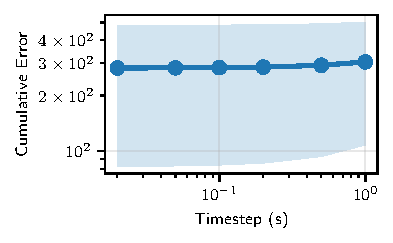
\includegraphics{plots/cumulative_error_pos_eta.pdf}
        \caption{Mean position error between surge and sway}
    \end{subfigure}
    \hspace{0.05\textwidth}
    \begin{subfigure}{0.45\textwidth}
        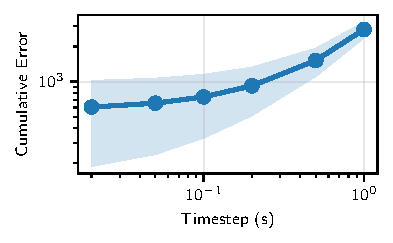
\includegraphics{plots/cumulative_error_rpm_fixed.pdf}
        \caption{RPM Error for fixed thrusters}
    \end{subfigure}
    \caption{Mean cumulative error per timestep size for position and thruster RPM. Error bar indicates variation between different realisations of the forcing process}
    \label{fig:timestep_difference}
\end{figure}

Time integration is done with a forward Euler scheme. The sensitivity of the model to timestep differences was
investigated. As a metric, the cumulative error between a benchmark timestep of \(0.01 s\) was taken. Runs of \(1000 s\) 
were used with 10 realisations of the stochastic forcing. Between timesteps, the forcing was kept the same. As shown
in \cref{fig:timestep_difference}, the position error is not sensitive to the timestep, whereas the thruster RPMs are
much more sensitive. For clarity, only the fixed thrusters are shown, but the bow thrusters follow the same trend. A
timestep of \(0.05 s\) is chosen to generate the training data.

To generate the training data, 50 realisations of Brownian motion were generated. The parameters used to generate the
external forces with the OU process are shown in \cref{tab:ou-params_pilot_test}.

\begin{table}[htbp]
    \centering
    \begin{tabular}{|c|c|}
        \hline
        \textbf{Term} & \textbf{Value} \\
        \hline
        \(\mu\) & \([75\cdot 10^3,\, 75\cdot 10^3,\, 100\cdot 10^3]\) \\        
        \(\sigma\) & \([50\cdot 10^3,\, 50\cdot 10^3,\, 50\cdot 10^3]\) \\
        \(\theta\) & \(0.01\) \\
        \hline
    \end{tabular}
    \caption{Ornstein-Uhlenbeck parameters used to generate training data}
    \label{tab:ou-params_pilot_test}
\end{table}

The initial position of the vessel is determined through uniform sampling between \(\pm 3 m\) for surge and sway and
\(\pm 0.15 rad\) for the yaw angle. The initial actuator actions are the result of the controller and thrust allocation
for the corresponding starting position.

The simulations were run for 3 simulated hours, corresponding to 216,000 timesteps. The process took 281.9 seconds, or
4.68 minutes. The runs were parallelised on the computer's CPU with 28 processes. 

\section{LatentSDE}
The first approach tested was neural SDEs. The LatentSDE method for training was chosen, as this is simpler to train
than the SDE-GAN approach \parencite{kidgerNeuralDifferentialEquations2022}. The Torch SDE package was used for these
initial tests. 

\subsection{Architecture}
The latent SDE consists of 5 neural networks: a prior drift network, a posterior drift network, a shared diffusion
network, an encoder for the measurements, and a decoder from the latent space to measurement space. 

The prior and posterior drift networks both consist of 3 linear layers, mapping a latent vector of dimension 4 into a
hidden dimension of 128. The activation function used between the linear layers is LipSwish
\parencite{kidgerNeuralDifferentialEquations2022}, a Lipschitz-continuous version of Swish or SiLU. A final hyperbolic
tangent activation was used to prevent the latent space from exploding during training
\parencite{kidgerNeuralSDEsInfiniteDimensional2021}. The posterior differs from the prior in that its input is
concatenated with a context vector of 64 that encodes the measurements.

The diffusion network is shared between the prior and posterior. As per the example provided in the TorchSDE, this is
implemented as a set of neural networks that result in a diagonal additive noise. Between the layers LipSwish is used, and a sigmoid function is used on the output.

The measurements are encoded using the encoder network. This consists of a gated recurrent unit (GRU) that takes the
entire time series of measured states and outputs a vector of 128 at every timestep. This is then passed through
a linear layer to make a context vector of 64 at each timestep.

The decoder is a single fully connected layer taking the latent vector of dimension 4 and mapping it to the state. The
state used is 12 dimensional. The values considered are \(\eta\), \(\nu\), and the thruster RPMs.

The initial state and observation noise distribution are also set as learnable parameters.

\subsection{Training and Evaluation}
The training is performed using the latentSDE approach developed by \textcite{liScalableGradientsStochastic2020} and
explained in \cref{subsubsec:latentsde}. During the forward pass of the network, an initial state is sampled. The
observation series is encoded. The posterior and prior networks are then integrated over time with an SDE solver, and
their adjoints are solved. The KL-divergence loss between the prior and posterior is calculated by augmenting the latent
state.

The SDE integration results in a generated series of latent vectors. These are passed through the decoder network. A
likelihood loss is then calculated between the generated series and the measured series. An additional KL-divergence
loss is calculated between the model's initial state and the data's initial state. The data's initial state is mapped
to a distribution in the latent space.

Training is done with the Adam optimiser. An exponential learning rate schedule was used with an initial rate of 0.005
and a decay ratio of 0.997. A linear KL schedule was used to ramp up the effect of the KL loss from 0 to full over 1000
epochs. Training was set to run over 5000 epochs. A timestep of 0.05 was used for the SDE integration, and a
period of 250 seconds was used, equating to a series of length 5000. A single file was used, resulting in a training set
of 40 time traces.

\begin{figure}[H]
    \centering
    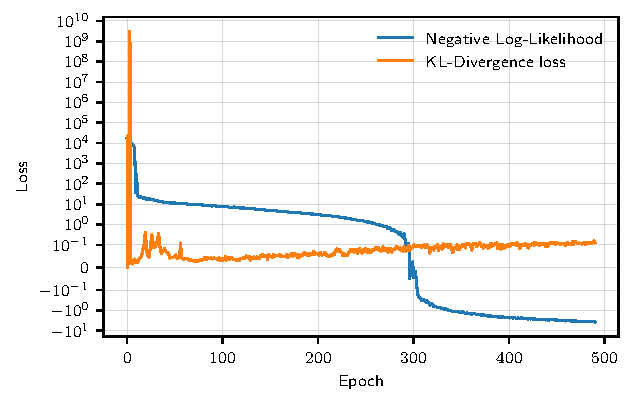
\includegraphics{plots/pilot_losses_latentsde.pdf}
    \caption{Training losses for LatentSDE training}
    \label{fig:pilot_latentsde_training}
\end{figure}


Training of the model was stopped after 492 epochs. This was after 17 hours and 49 minutes. Figure
\cref{fig:pilot_latentsde_training} shows the training losses per epoch. As can be seen, the reconstruction loss at the
end of training is very small, with the log-likelihood becoming negative. The KL-divergence loss is in a similar order
of magnitude, though still rising. This can be attributed to the KL annealing not fully including the loss yet at 491
epochs. The prior was sampled and integrated over a period of 250 seconds. The generated traces of the surge motion are shown in \cref{fig:pilot_latentsde_generation}. 

\begin{figure}[H]
    \centering
        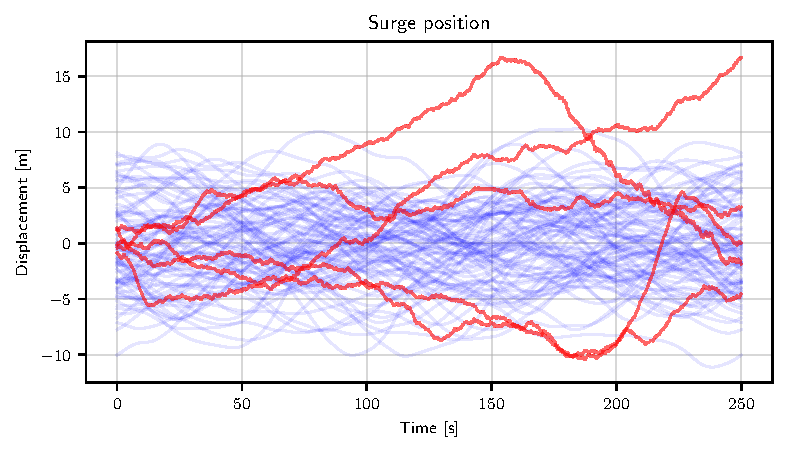
\includegraphics{plots/pilot_latentSDE.pdf}
    \caption{Generated surge motions (Red) and training trajectories (Blue)}
    \label{fig:pilot_latentsde_generation}
\end{figure}

While the trajectories themselves are by no means accurate representations of the training data, they do show some
promise for the desired application. The traces show the model has managed to learn the magnitude of the motions for
this integration period. Some of the traces exhibit expected behaviour of a DP system in their return to zero. 

There are several caveats. The reconstructed traces are generated from the prior network. The model training was stopped
after 492 epochs, meaning the contribution of the KL loss was not fully included yet. As the KL loss is the primary loss
driving the training of the prior, the prior has not been trained to the same extent as the posterior. Second, the
training took a very long time for the size of the training set and the length of the time series.

Inference of the model also took a significant amount of time. For the five traces shown in
\cref{fig:pilot_latentsde_generation}, TorchSDE took 937 seconds. A manual test was performed to investigate the cause.
An Euler-Maruyama integration loop was set up, and the model's prior diffusion network and drift network were sampled
directly. The test was run for the same size and length as the toy model training data: 50 batches for 10,800 seconds
with a timestep of 0.05 s. The result was the model taking 161 seconds to complete the run. This was performed with a
single CPU core, with the models running in parallel on the GPU. As such, the time increase with respect to an increased
batch size does not increase linearly. The cause of the speed difference between TorchSDE and the manual approach is
unknown at the time of writing. Overall, the manual test showed a speed increase of 1.75x with respect to the toy model.

\section{DeepONet}
The second approach tested was DeepONet. For these tests, the multiple input operator network described in
\textcite{jinMIONetLearningMultipleInput2022} is used. The networks are built upon the PyTorch implementation used by
\textcite{moyaDeepONetgridUQTrustworthyDeep2023} in their work on uncertainty quantification with DeepONets.

\subsection{Architecture}

The MIONet approach uses a separate branch network per input function. The inputs used are the external stochastic force
and an initial position. The branch nets consist of two types: the initial condition is encoded using two linear layers,
whereas the force traces are encoded using 1-dimensional convolutional layers. \Cref{fig:mionet_architecture} gives a
graphical representation as well as the dimensions of each layer.

\begin{figure}[H]
    \centering
    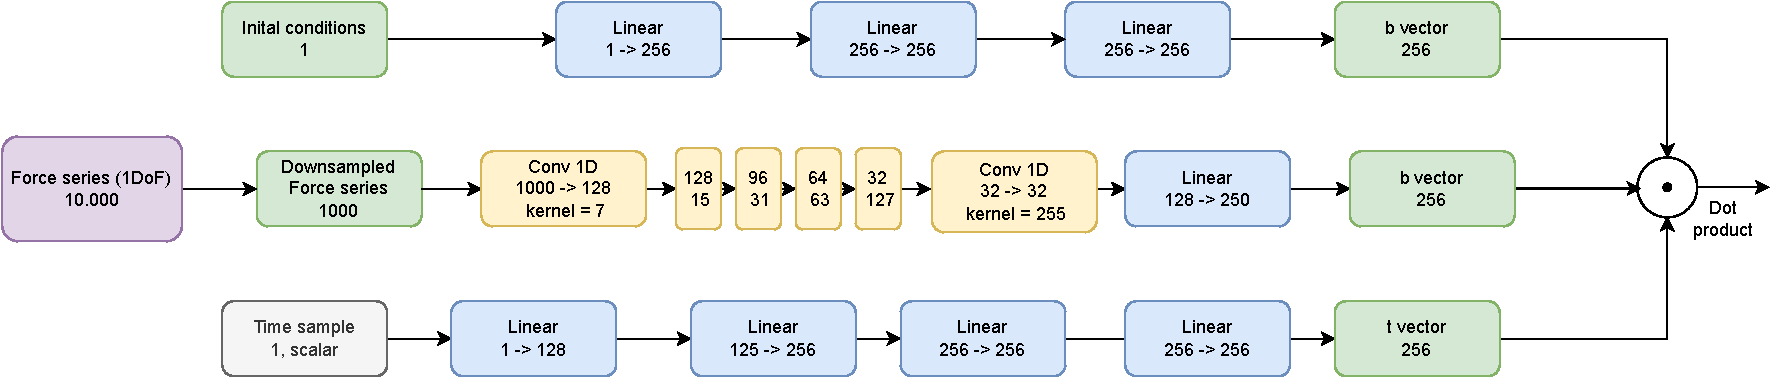
\includegraphics[width=\linewidth]{report/images/diagrams/1dof_mionet.pdf}
    \caption{MIONet architecture used (1 degree of freedom)}
    \label{fig:mionet_architecture}
\end{figure}

Each convolutional layer in \cref{fig:mionet_architecture} consists of a convolution and a dropout layer with a dropout
rate of 0.1. All the branch layers used the GeLu activation function. The initial condition was passed to a branch
network and the force series to another. The force was downsampled to a timestep of 0.5 seconds.

\subsubsection{Training and Evaluation}

Training was performed on series of the training sets subsampled to be 10000 items long. These were then sampled every
0.5 seconds to give a series of 1000 measurements. Before training and testing, the dataset was scaled using the mean
and standard deviation of each individual feature. The time was scaled between 0 and 1. Training was performed over
1350 epochs. An initial learning rate of 0.01 was used with a schedule to reduce it on a plateau of test loss. A sample
size of 2048 random timesteps was used to train and test. An 80-20 training testing data split was used. 

DeepONet was first tested with a 1 degree of freedom case. A new dataset was generated from the toy model with pure
surge force and motion. 100 different seeds were used. Before training the time series was normalised to be between 0
and 1, and the input feature was normalised to have a mean of 0 and a standard deviation of 1.

\begin{figure}[H]
    \centering
    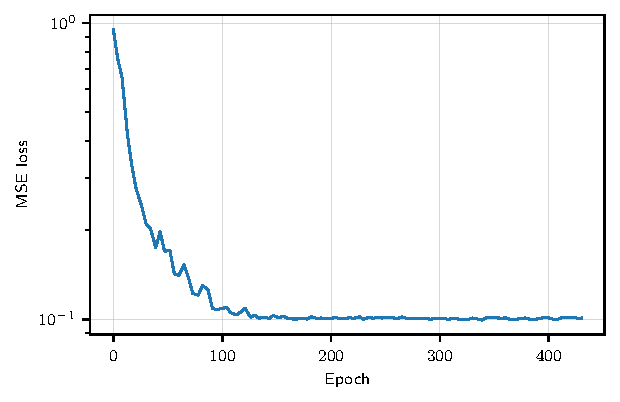
\includegraphics{plots/pilot_losses_deepOnet.pdf}
    \caption{Testing loss for 1 DoF DeepONet. Figure is capped at 400 epochs for clarity}
    \label{fig:pilot_deeponet_test_loss}
\end{figure}

\Cref{fig:pilot_deeponet_test_loss} shows the training losses of the operator network. After \approx 250 epochs the loss
flattens out. It does not drop below 0.1 past this point. \Cref{fig:deeponet_pilot} shows a reconstructed time
trace for the surge motion. 

\begin{figure}[H]
    \centering
    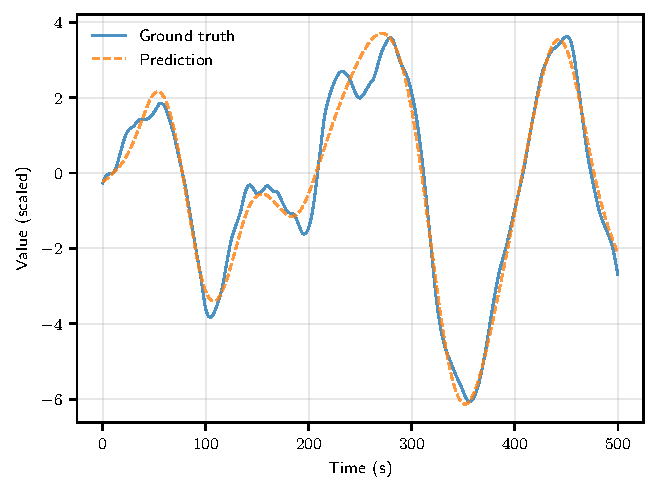
\includegraphics{plots/pilot_deepOnet_1dof.pdf}
    \caption{Randomly selected surge reconstruction of 1 DOF DeepONet. Both axes are normalised}
    \label{fig:deeponet_pilot}
\end{figure}

As can be seen in \cref{fig:deeponet_pilot}, the network appears capable of reconstructing the vessel motions given a
force time history as input. In particular, the large, lower frequency motions are captured best. Some of the smaller,
sharper oscillations are not captured as accurately. Inference of the model takes a negligible about of time, marking a
significant speed-up compared to the toy model. This is however only a 1 dimensional case, how the method scales to
higher degrees of freedom is not yet known.

\section{Conclusion}
Both the experiments show capability of the researched methods for simulating the dynamics of a stochastically excited
DP system. As such, the decision on which to use comes down to their suitability to real world use. 

Assuming their performance issue can be overcome, neural SDEs offer more flexibility for
use in practice, as they do not require a fixed sample length or interval, or generation of a force series for training.
This makes the approach more suitable for real-world applications where data is not guaranteed to be perfectly sampled. 
As such neural SDEs will be used moving forward in this research.

